
\chapter{Test af equalizer}\label{sec:test_eq}


\begin{figure}[h]
	\vspace*{-1 cm}
	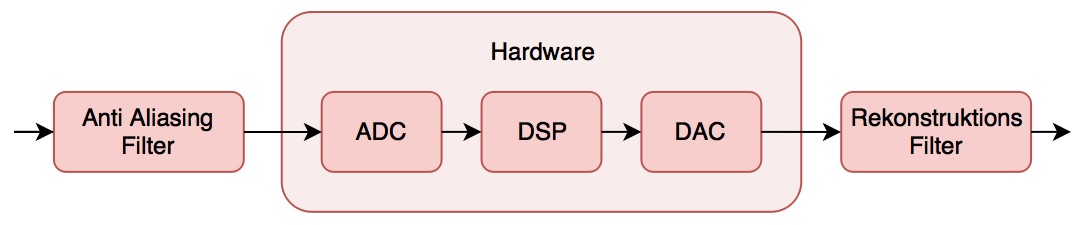
\includegraphics[width=8cm]{billeder/flow_all}
	\vspace{0.5 cm}
\end{figure}


\emph{I dette kapitel bliver der redegjort for testforløbet af equalizeren. Der bliver brugt en Bode 100 til måling af equalizerens overførselsfunktion. På denne måde kan det bevises om equalizerens profiler fungerer korrekt.}

\section{Forberedelse}


For bedst at teste equalizeren, blev der besluttet at følgende tre 3 parametre skulle gennemtestes: 

\begin{enumerate}[noitemsep,nolistsep]
    \item Amplituden/Gain
    \item Bandwidth
    \item Frekvens \\
\end{enumerate}



Under disse parametre var der en del forskellige ting der skulle tages højde for. 
\begin{enumerate}[noitemsep,nolistsep]
    \item Ved amplituden skulle der holdes en fast bandwidth ($100\hertz$) og en fast frekvens ($1\kilo\hertz$). Der blev målt hhv. $\pm5\decibel$ og $\pm7\decibel$
    \item Ved bandwidth skulle der holdes en fast amplitude ($\pm5\decibel$) samt en fast frekvens. ($1\kilo\hertz$). Her blev der målt forskellig bandwidth, hhv. $100\hertz$, $500\hertz$ og $1\kilo\hertz$.
    \item Ved frekvensen blev der holdt en fast amplitude ($\pm5\decibel$) og fast bandwidth ($100\hertz$). Her blev der dog målt med forskellige typer filtre. Peak filtret blev målt ved $100\hertz$ og $5\kilo\hertz$, hvor high shelf og low shelf filtrene blev målt ved $1\kilo\hertz$ og $5\kilo\hertz$. \\
\end{enumerate}

Derudover blev der opstillet en "kode-test" hvor der blev beregnet filtre som alle havde samme egenskaber, uanset om dette var et peak, high shelf eller et low shelf. Dette var for at eftervise om DSP koden var konsistent i alle typer filtre. \\

\section{Udførelse}
For at måle overføringsfunktionen sættes Bode 100'ens output til indgangen på equalizeren. CH1 sættes også til indgangen. CH2 sættes til udgangen og målingen foretages for samtlige af ovenstående presets. Bodens udgangslevel sættes til $-4\decibel\milli$, for at undgå overstyring uanset profil. CH1 og CH2's dæmpning sættes til $0\decibel$ og der måles fra $20\hertz$ til $20\kilo\hertz$ da dette er det normale lydområde.\\


\begin{figure}[h!]\label{fig:bode_setup}
	\centering
	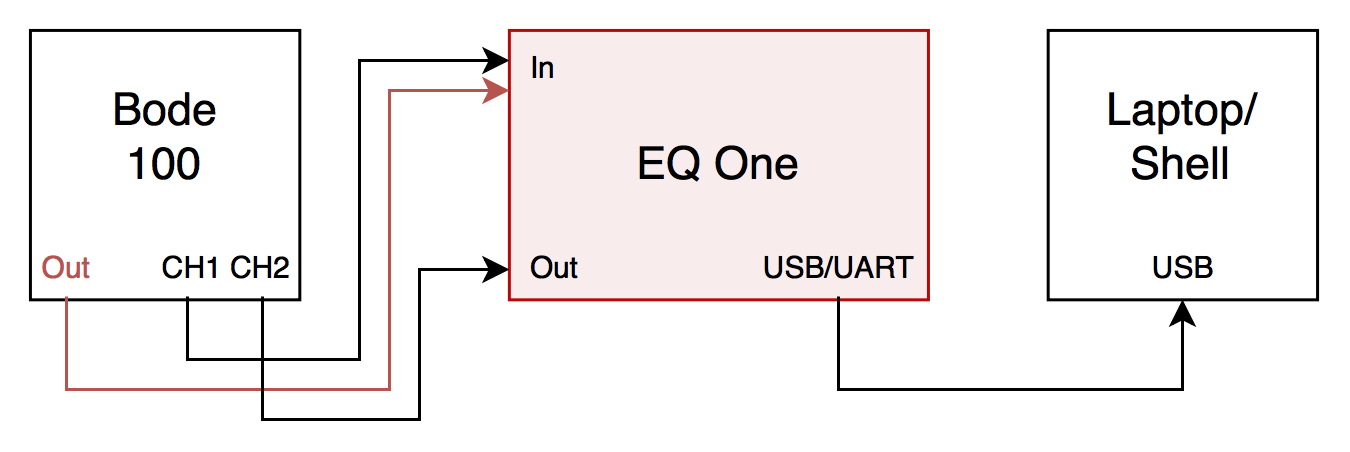
\includegraphics[width=0.7\textwidth]{billeder/bode_setup}
	\caption{Målingeopstilling af equalizer med Bode 100}
\end{figure}	

\FloatBlock

\section{Resultater}
I dette afsnit vil resultaterne af målingerne blive vist, og der vil herefter drages til delkonklusion, hvor teorien stilles op mod praktis.
Det første resultat på figur \ref{fig:eq_off1}, viser en graf hvor den digitale del er slået fra, og selve equalizeren er deaktiveret. Det er altså kun de analoge filtre der dominerer. Da der hovedsageligt testes om profilerne fungerer, altså om DSP koden er korrekt, trækkes denne "afvigelse" fra målingerne, så disse bliver så tæt på teorien som muligt. Det teoretiske AA-filter ses til sammenligning på figur \ref{fig::anfilter_sim_total}, hvor det stemmer overens med målingen.

\begin{figure}[h!]
	\centering
	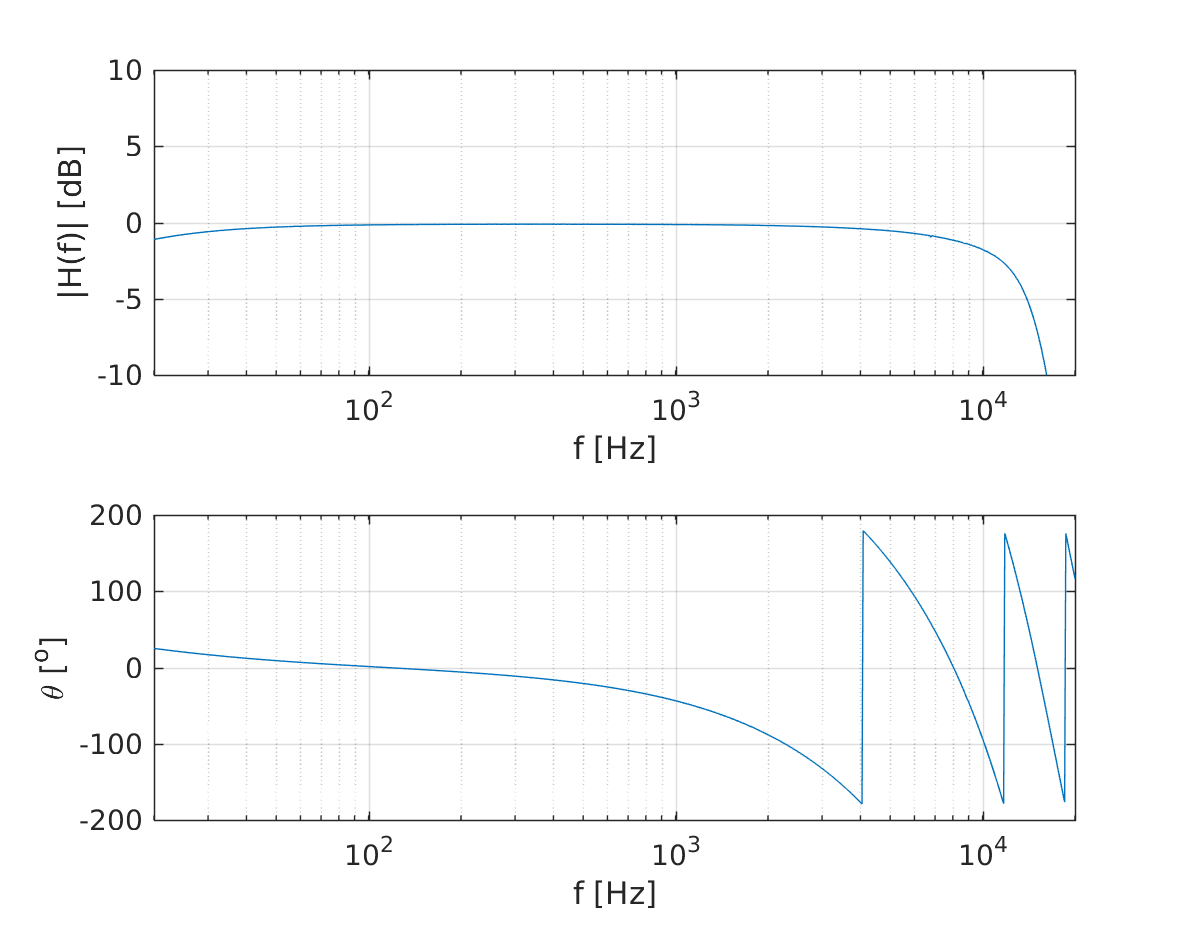
\includegraphics[width=10cm]{matlabdemo/test/test_eq_off.png}  
	\caption{Måling af hele systemet uden equalizer slået til.}
	\label{fig:eq_off1}
\end{figure}

Den vigtige del at eftervise, er hvor equalizeren er slået til. 
Udfra forberedelsen, skulle 3 parametre testes - amplituden, båndbredden og frekvensen. 
Da der blev målt første gang, viste det sig, at både frekvensen og båndbredden afvigede med ca. en faktor 2, hvorfor der blev lavet en måling med korrigerede parametre. Amplituden afvigede i det positive spektrum med ca. 1.75, og i det negative med ca. 3.75, hvilket også blev korrigeret. Disse faktorer blev fundet ved hjælp af "trial and error"-metoden (læs: prøve-fejl-metode) ved de forskellige profiler. \\
De teoretiske beregninger og resultater stilles op ved siden af hinanden.
Dette ses for hhv. hver parameter i figur: \ref{fig:gain}, \ref{fig:bw} og \ref{fig:freq}. 
Her ses tydeligt den afvigende amplitude og båndbredde, som beskrevet tidligere. På figur \ref{fig:korr} ses de korrigerede målinger.

\subsection{Målinger}

\begin{figure}[h!]
	\vspace*{-0.3 cm}
	\centering
	\subbottom[]{%
	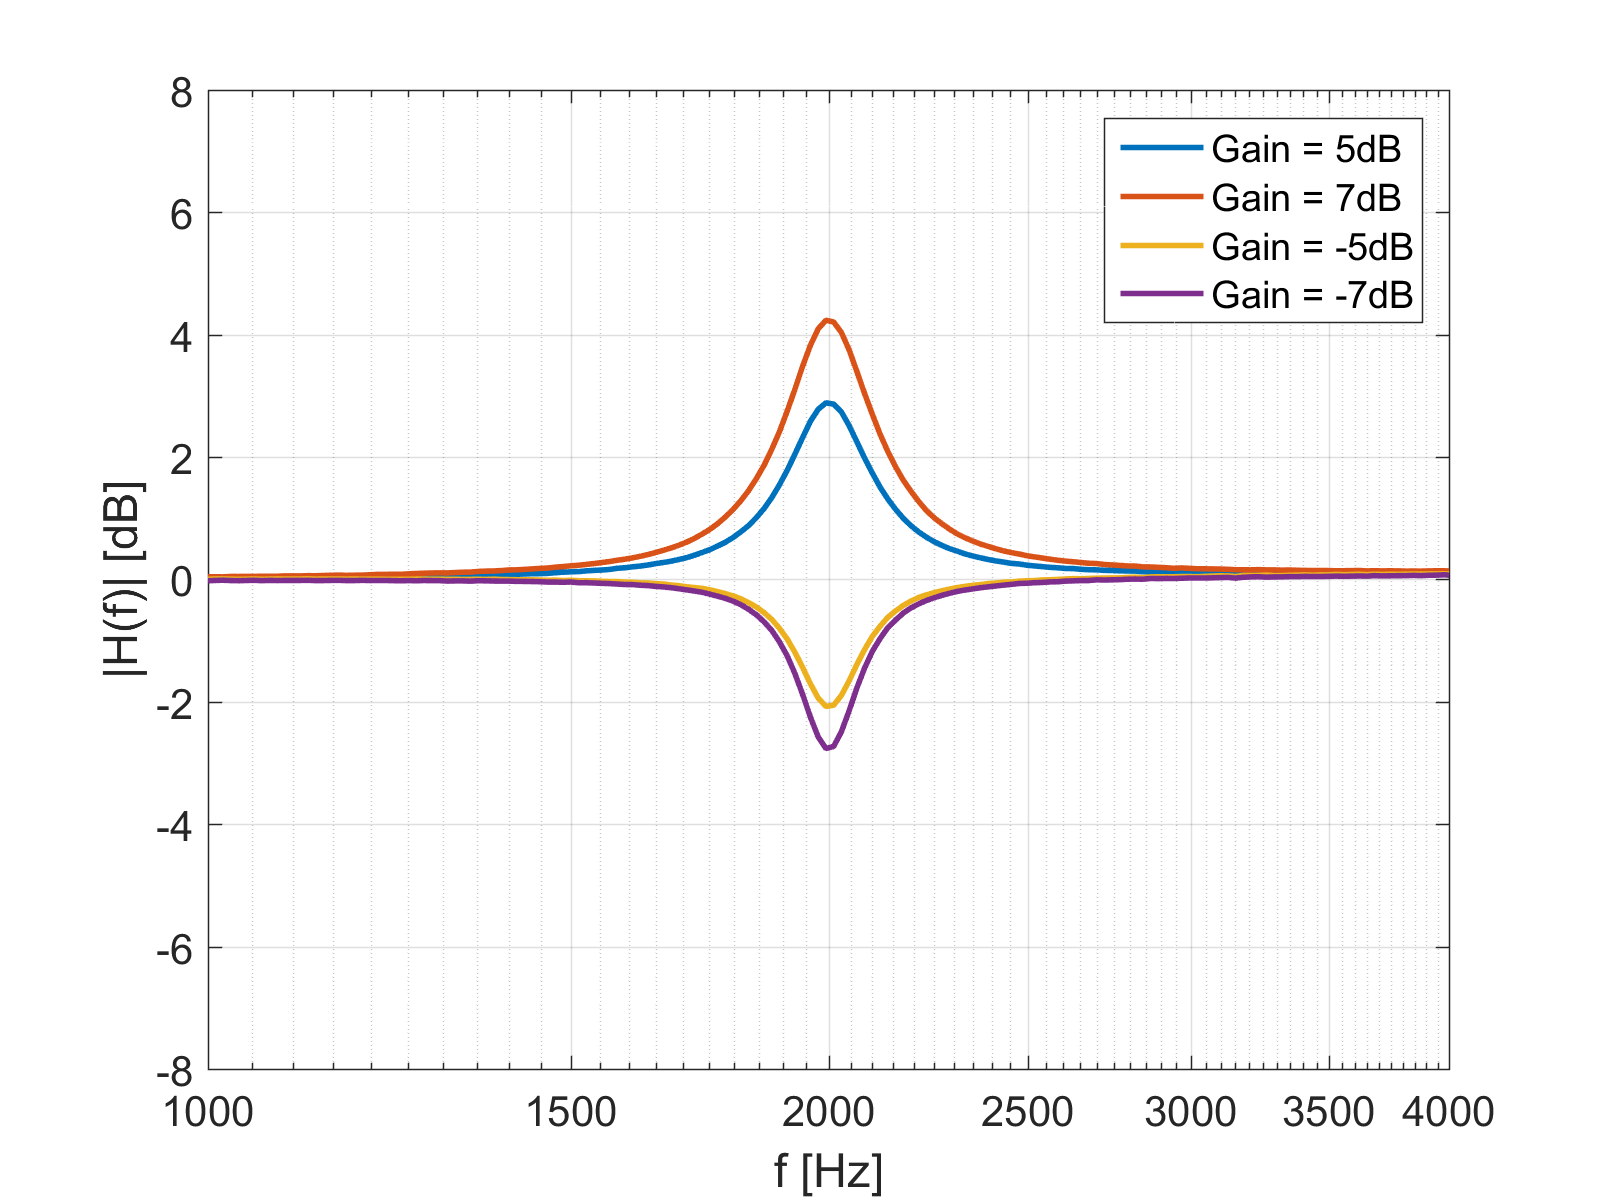
\includegraphics[width=0.47\textwidth]{billeder/gain_meas}
	\label{fig:gain_uden_hotfix}}
	\subbottom[]{%
	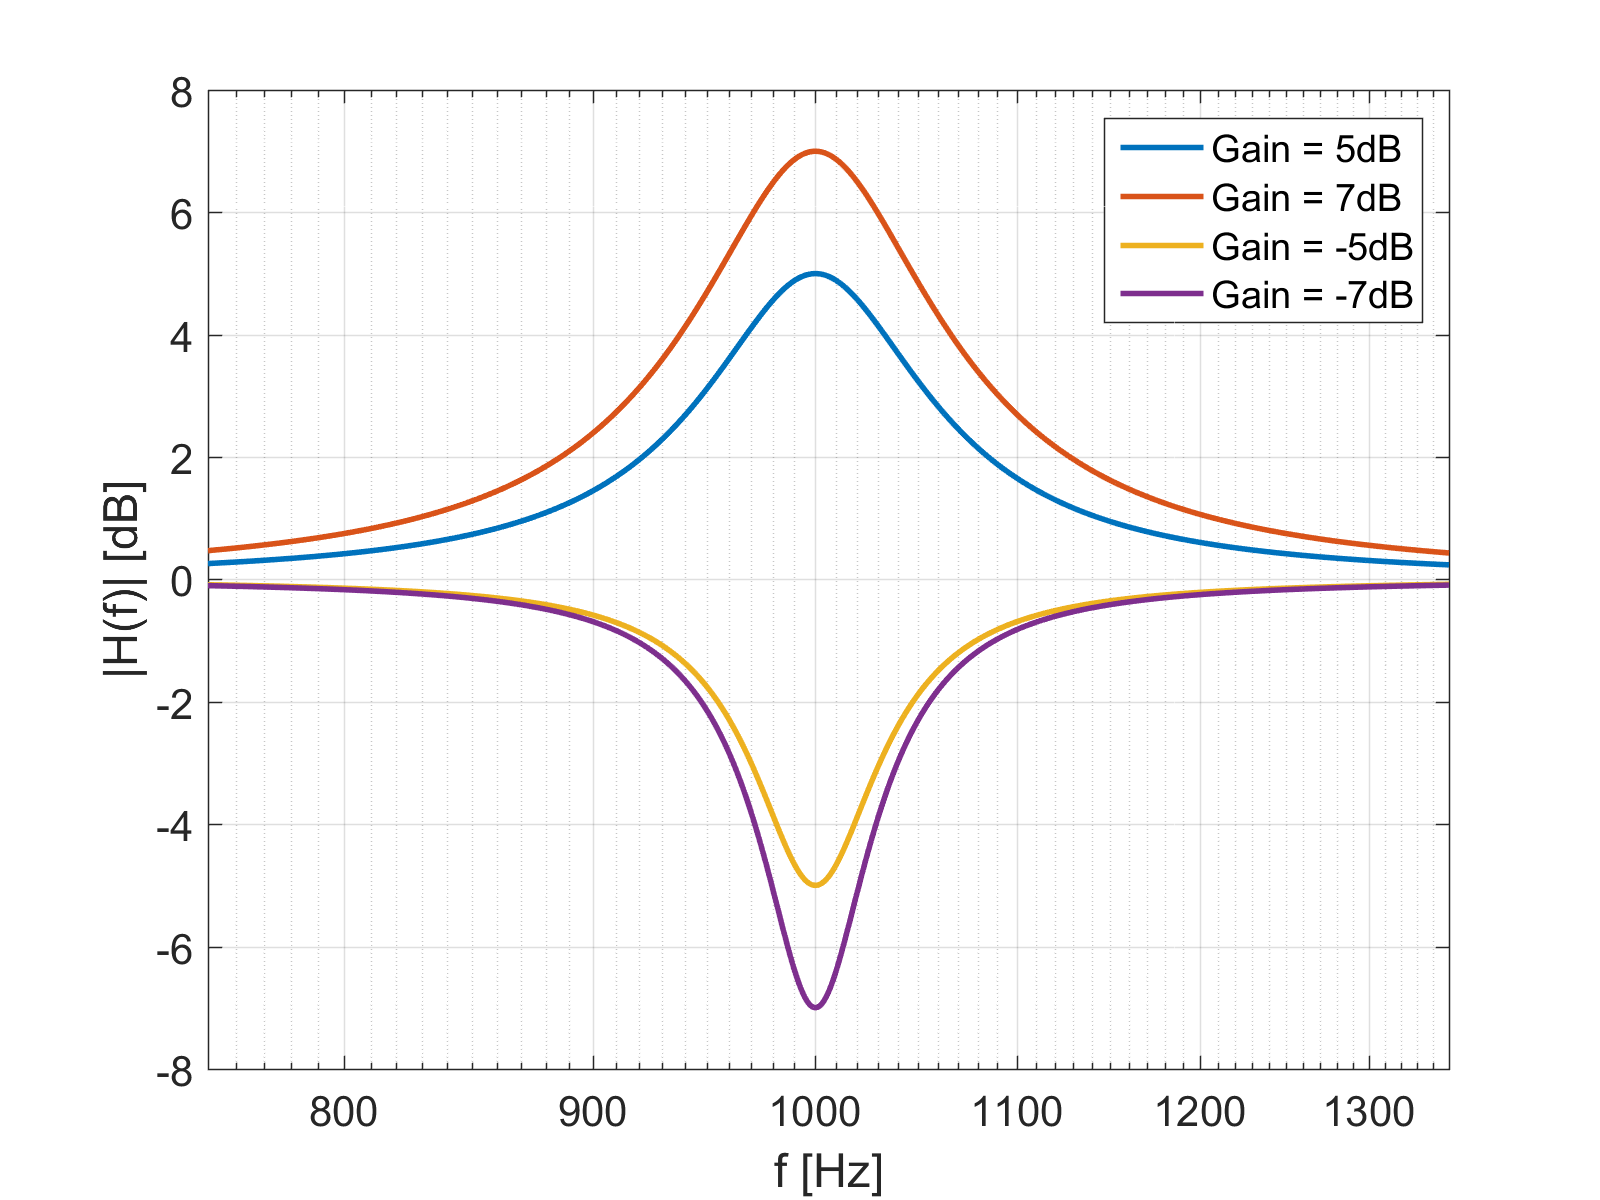
\includegraphics[width=0.47\textwidth]{billeder/gain_teori}
	\label{fig:gain_teori}}
  	\caption{Målingsresultat af gain ($\pm5\decibel$ og $\pm7\decibel$, figur \ref{fig:gain_uden_hotfix}) sammenlignet med teorien (\ref{fig:gain_teori})}
	\label{fig:gain}
\end{figure}

\begin{figure}[h!]
	\vspace*{-0.3 cm}
	\centering
	\subbottom[]{%
	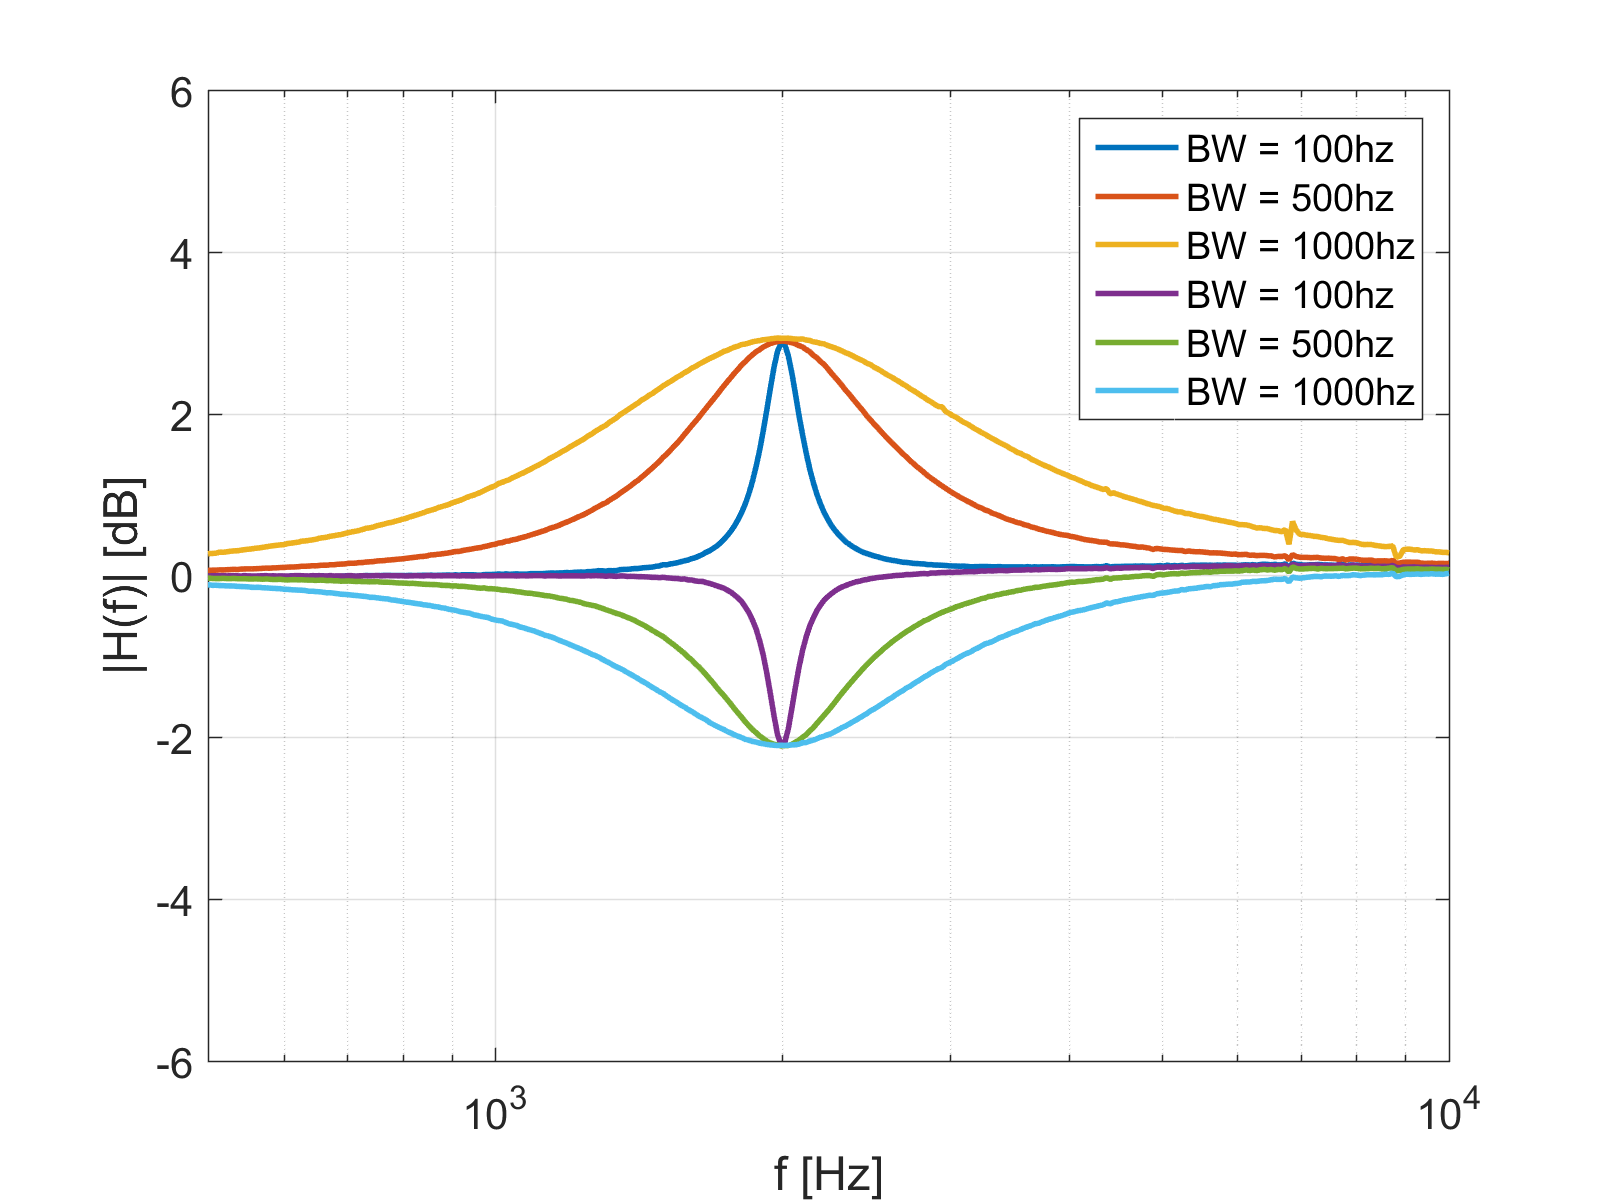
\includegraphics[width=0.47\textwidth]{billeder/bandwidth_meas}
	\label{fig:bandwidth_uden_hotfix}}
	\subbottom[]{%
	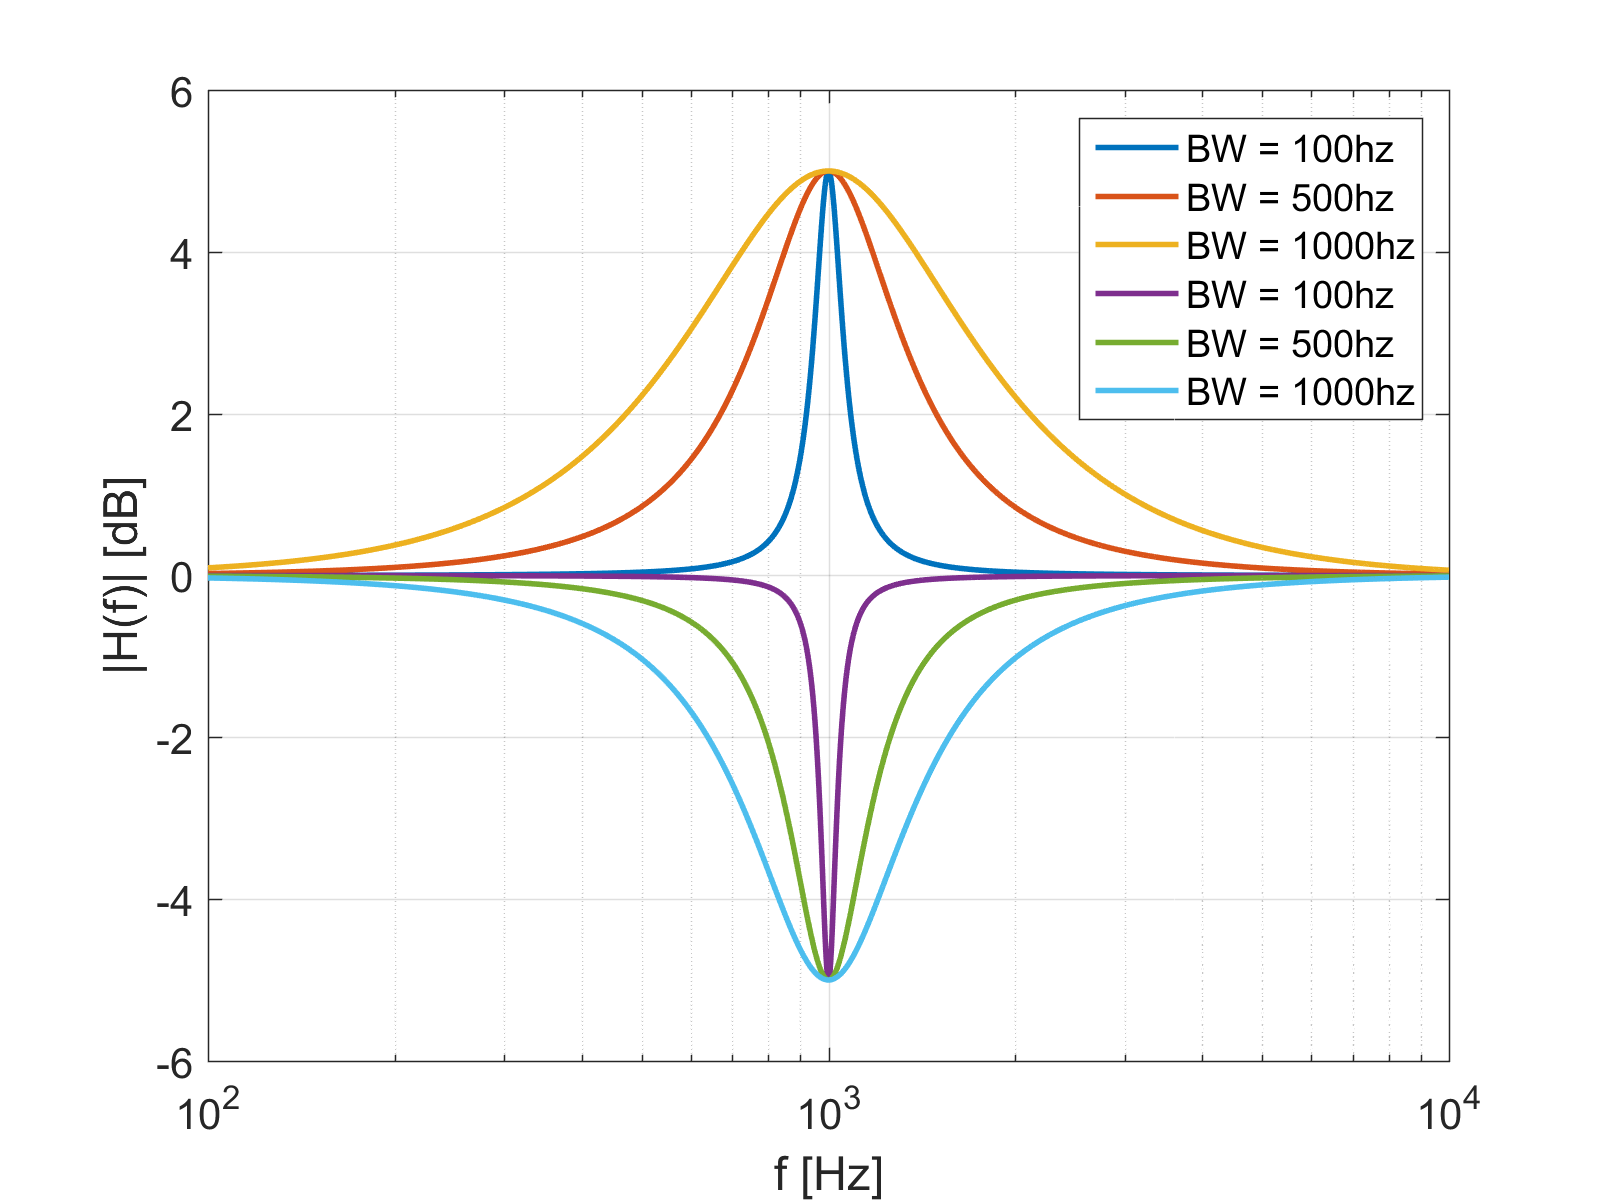
\includegraphics[width=0.47\textwidth]{billeder/bandwidth_teori}
	\label{fig:bandwidth_teori}}
  	\caption{Målingsresultat af forskellig bandwidth (hhv. $100\hertz$, $500\hertz$ og $1\kilo\hertz$, figur \ref{fig:bandwidth_uden_hotfix}), sammenlignet med teorien (\ref{fig:bandwidth_teori}.}
	\label{fig:bw}
\end{figure}

\begin{figure}[h!]
	\vspace*{-0.3 cm}
	\centering
	\subbottom[]{%
	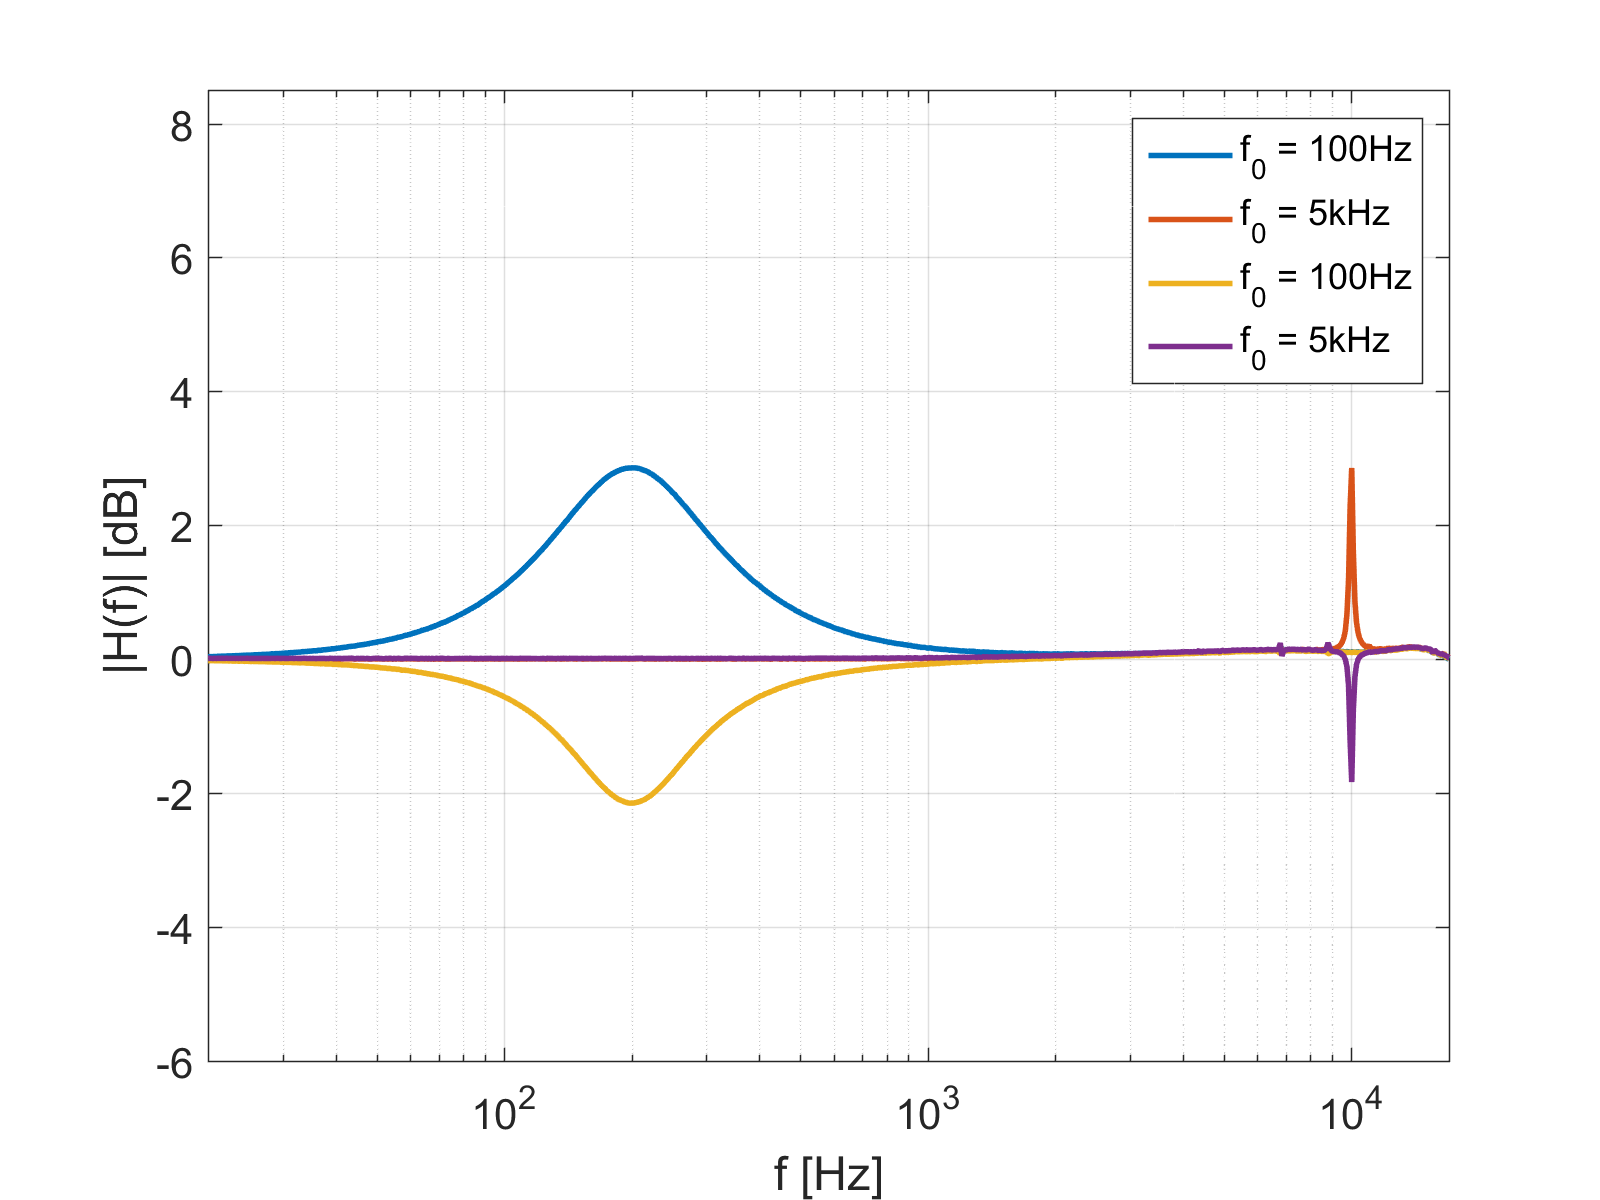
\includegraphics[width=0.47\textwidth]{billeder/frekvensplacering_meas}
	\label{fig:freq_uden_hotfix}}
	\subbottom[]{%
	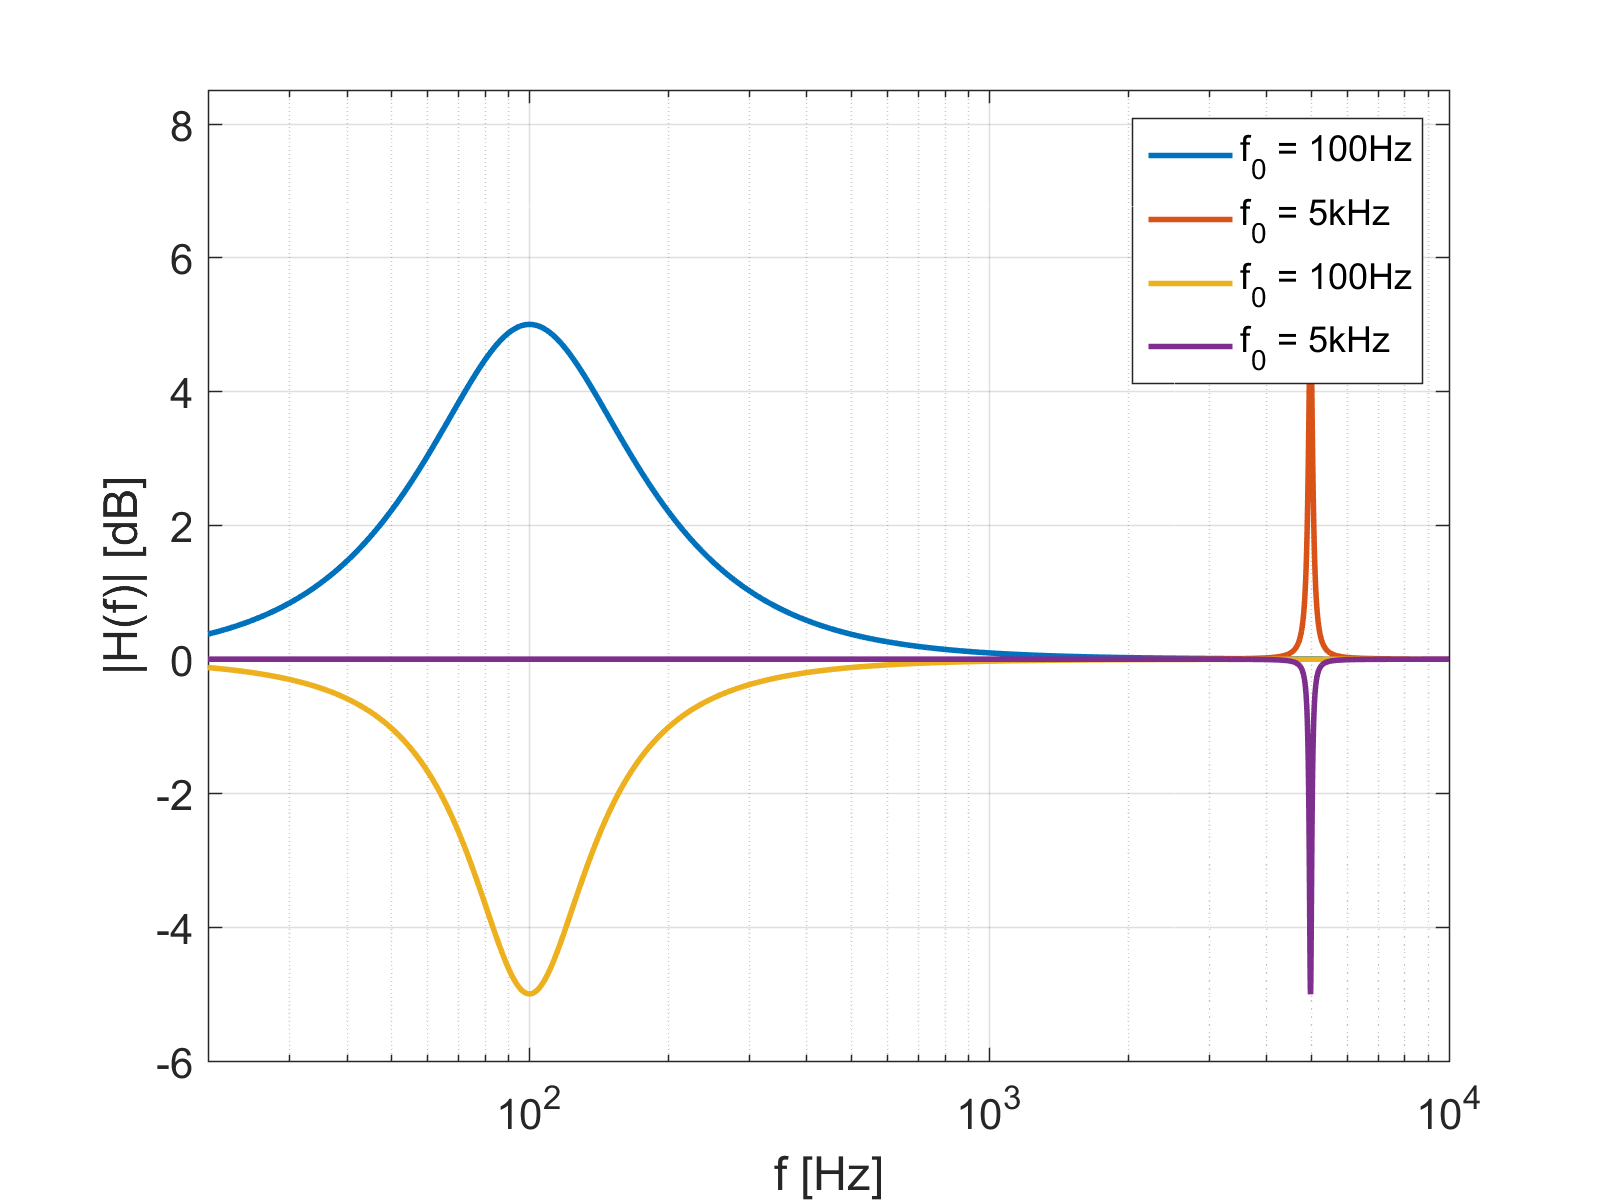
\includegraphics[width=0.47\textwidth]{billeder/frekvensplacering_teori}
	\label{fig:freq_teori}}
  	\caption{Målingsresultat af forskellig frekvens (hhv. $100\hertz$ og $5\kilo\hertz$, figur \ref{fig:freq_uden_hotfix}), sammenlignet med teorien (\ref{fig:freq_teori}.}
	\label{fig:freq}
\end{figure}

\begin{figure}[h!]
	\centering
	\subbottom[]{%
	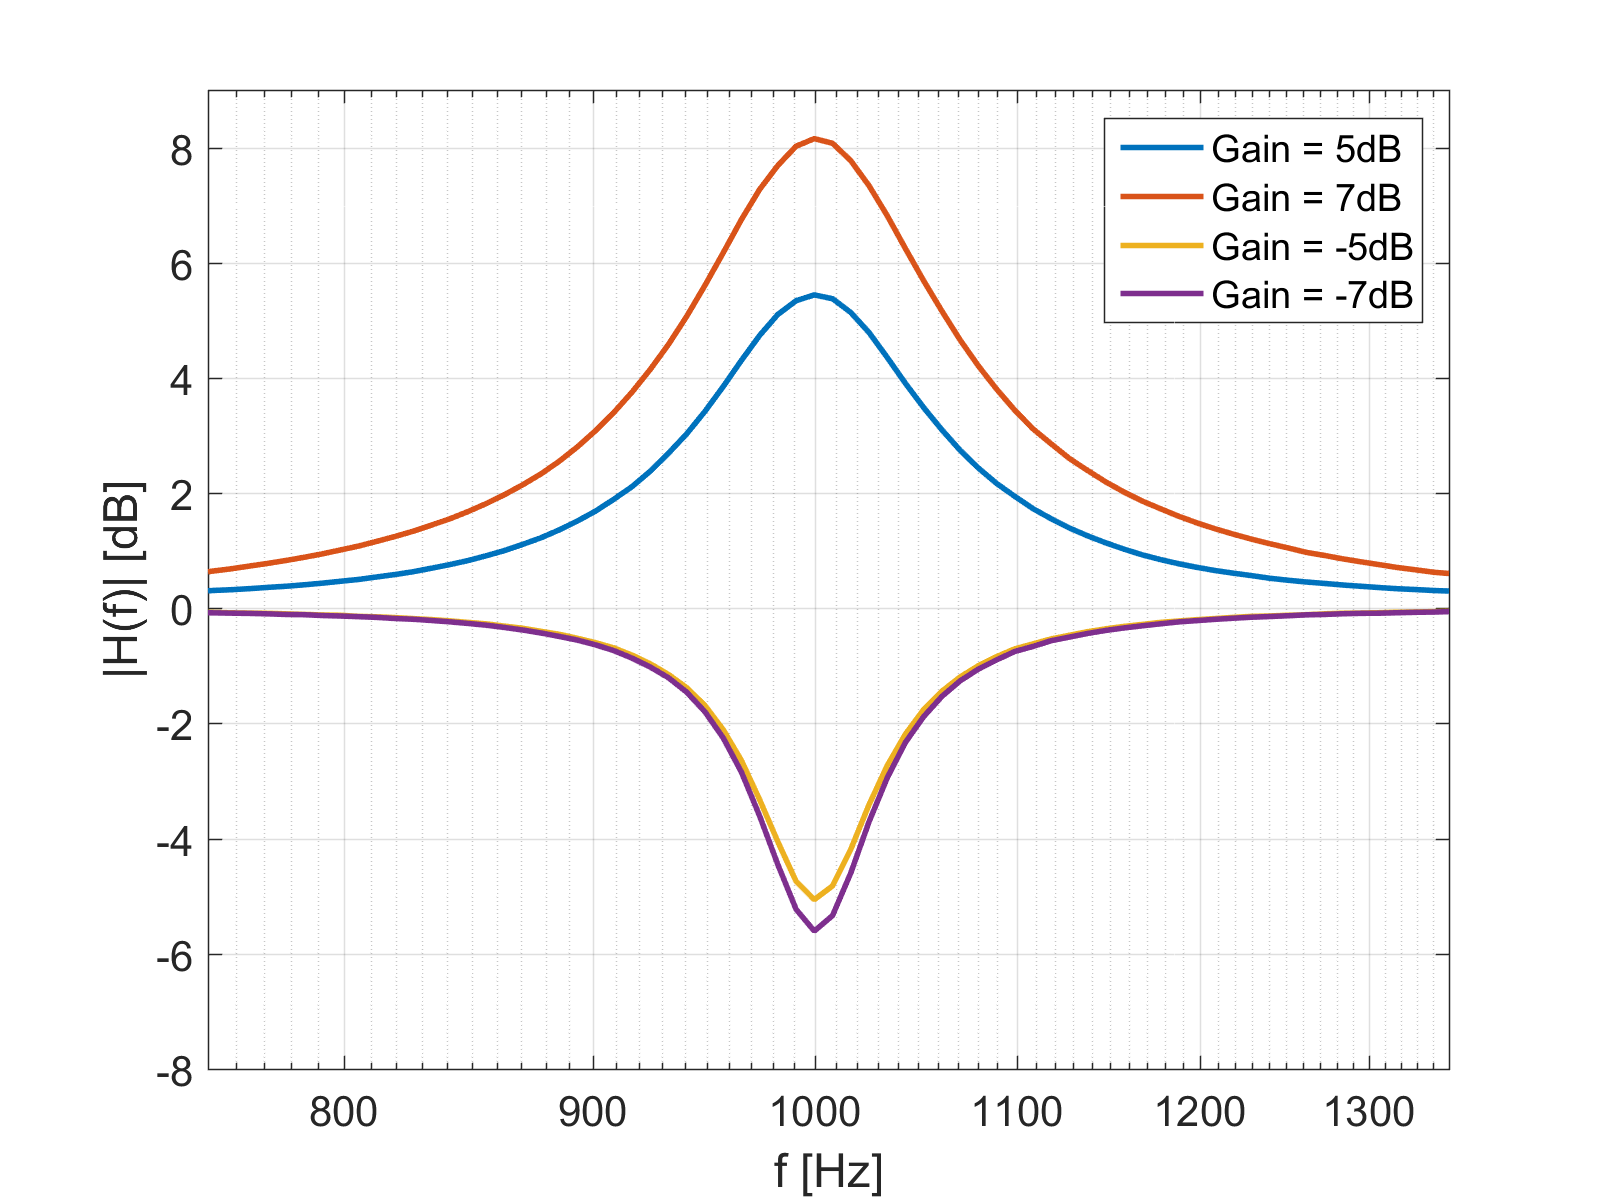
\includegraphics[width=0.47\textwidth]{billeder/gain_meas_med_hotfix}
	\label{fig:gain_med_hotfix}}
	\subbottom[]{%
	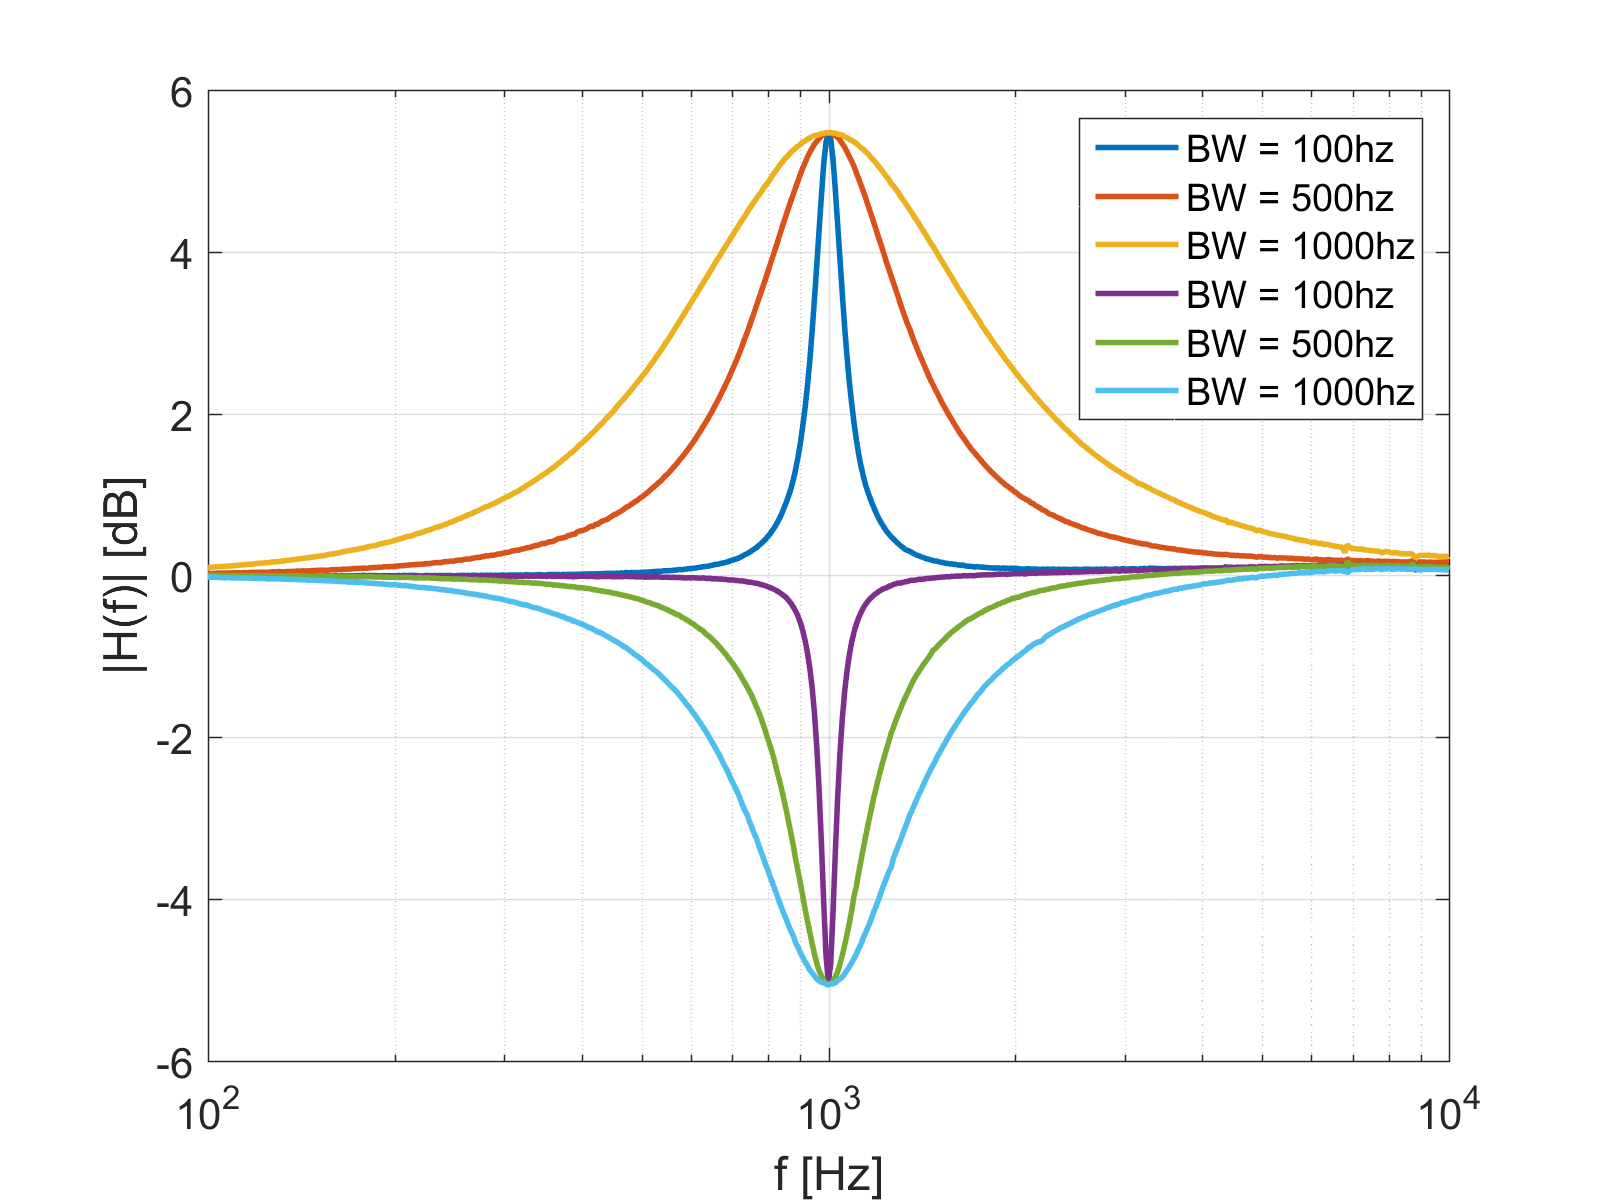
\includegraphics[width=0.47\textwidth]{billeder/bandwidth_meas_med_hotfix}
	\label{fig:bandwidth_med_hotfix}}
	\subbottom[]{%
	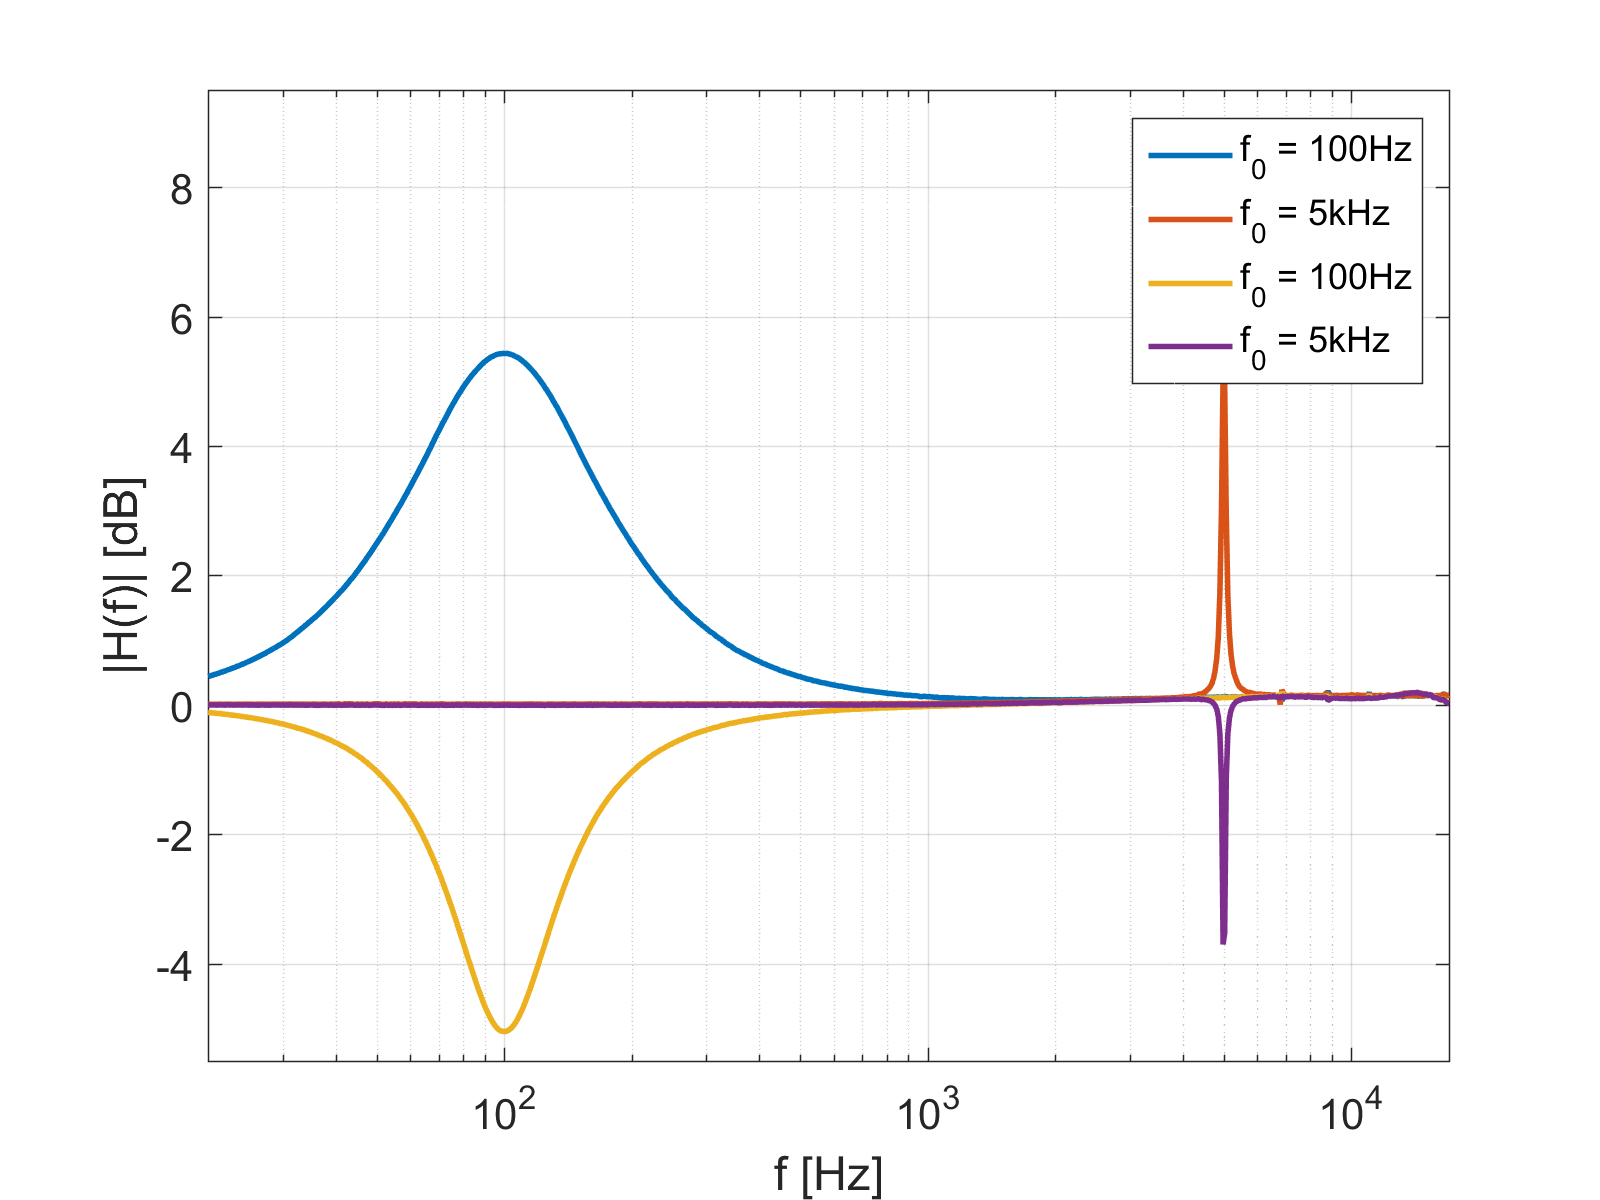
\includegraphics[width=0.47\textwidth]{billeder/frekvensplacering_meas_med_hotfix}
	\label{fig:frekvensplacering_med_hotfix}}
  	\caption{Her ses de korrigerede målinger for hhv. gain (\ref{fig:gain_med_hotfix}), bandwidth (\ref{fig:bandwidth_med_hotfix}) og frekvens (\ref{fig:frekvensplacering_med_hotfix}).}
	\label{fig:korr}
\end{figure}

Da der er anvendt bilinær transformation, er det kun centerfrekvensen der er garanteret, at være korrekt.
Dette ses også i forhold til figur \ref{fig:freq}, hvor båndbredden ses at være mindre i det negative gain. 

\section{Delkonklusion}

Ved hjælp af disse tests kan, der konkluderes at de forskellige parametre som indstilles i koden kommer til at passe på udgangene. Der blev også bevist at de matematiske beregninger, altså DSP implementeringen, passer med teorien og at filtrene opfører sig som forventet. \\

Disse tests var derudover med til at finde nogle enkelte småfejl/offsets som gjorde at frekvensen, båndbredden samt amplituden ikke lå helt hvor de skulle. Disse faktorer blev fundet ved at sammenligne Bode 100 målingerne med de teoretiske beregninger, og derefter bruge "trial and error"-metoden til at finde de korrekte værdier. Årsagen til dette offset kendes endnu ikke, men tests'ene beviste at de ikke lå i matematikken, men andetsteds. 
Beviset for dette, er gjort ved at bruge de beregnede koefficienter fra MATLAB, og implmentere dem direkte i DSP modulet. Dette viste de samme målinger efterfølgende, og det kan dermed konkluderes at teorien er korrekt.











